\tikzset{%
  input/.style={
      circle,
      draw,
      color={rgb, 255:red, 107; green, 65; blue, 144 },
      draw opacity=1,
      fill={rgb, 255:red, 107; green, 65; blue, 144 },
      fill opacity=0.48,
      minimum size=0.5cm
    },
    every neuron/.style={
      circle,
      draw,
      color={rgb, 255:red, 65; green, 117; blue, 5 },
      draw opacity=1,
      fill={rgb, 255:red, 65; green, 117; blue, 5 },
      fill opacity=0.48,
      minimum size=0.5cm
    },
    neuron missing/.style={
      draw=none, 
      fill=none,
      scale=1,
      text height=0.333cm,
      execute at begin node=\color{black}$\vdots$
    },
    output/.style={
      circle,
      draw,
      color={rgb, 255:red, 107; green, 65; blue, 144 },
      draw opacity=1,
      fill={rgb, 255:red, 107; green, 65; blue, 144 },
      fill opacity=0.48,
      minimum size=0.5cm
    },
}
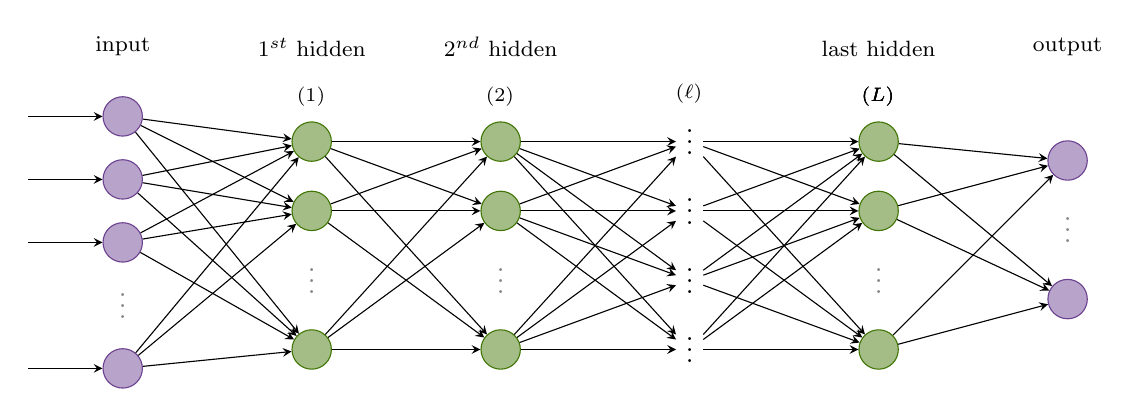
\begin{tikzpicture}[x=1.2cm, y=0.8cm, >=stealth]

\foreach \m/\l [count=\y] in {1,2,3,missing,4}
  \node [input/.try, neuron \m/.try] (input-\m) at (0,2.2-\y) {};

\foreach \m [count=\y] in {1,2,missing,3}
  \node [every neuron/.try, neuron \m/.try ] (firsthidden-\m) at (2,1.9-\y*1.1) {};

\foreach \m [count=\y] in {1,2,missing,3}
  \node [every neuron/.try, neuron \m/.try ] (secondhidden-\m) at (4,1.9-\y*1.1) {};

\foreach \m [count=\y] in {1,2,3,4}
  \node [neuron missing/.try, neuron \m/.try ] (thirdhidden-\m) at (6,1.9-\y*1.1) {};

\foreach \m [count=\y] in {1,2,missing,3}
  \node [every neuron/.try, neuron \m/.try ] 
(lasthidden-\m) at (8,1.9-\y*1.1) {};

\foreach \m [count=\y] in {1,missing,2}
  \node [output/.try, neuron \m/.try ] 
(output-\m) at (10,1.6-\y*1.1) {};



\foreach \l [count=\i] in {1,2,3,n}
  \draw [<-] (input-\i) -- ++(-1,0);
  \node [above] at (input-1.north) {$\bx$};

\foreach \l [count=\i] in {1};
\node [above] at (firsthidden-1.north) {$\bh^{(1)}$};

% \foreach \l [count=\i] in {1,2,n}
%   \node [above] at (secondhidden-\i.north) {$h^{(2)}_\l$};

\foreach \l [count=\i] in {1};
  \node [above] at (secondhidden-1.north) {$\bh^{(2)}$};

\foreach \l [count=\i] in {1}
  \node [above] at (thirdhidden-1.north) {$\bh^{(\ell)}$};

\foreach \l [count=\i] in {1,2,n}
%   \draw [->] (lasthidden-\i) -- ++(1,0);
 \node [above] at (lasthidden-1.north) {$\bh^{(L)}$};

\foreach \l [count=\i] in {1}
  \node [above] at (output-1.north) {$\by$};



\foreach \i in {1,...,4}
  \foreach \j in {1,...,3}
    \draw [->] (input-\i) -- (firsthidden-\j);

\foreach \i in {1,...,3}
  \foreach \j in {1,...,3}
    \draw [->] (firsthidden-\i) -- (secondhidden-\j);

\foreach \i in {1,...,3}
  \foreach \j in {1,...,4}
    \draw [->] (secondhidden-\i) -- (thirdhidden-\j);

\foreach \i in {1,...,4}
  \foreach \j in {1,...,3}
    \draw [->] (thirdhidden-\i) -- (lasthidden-\j);

\foreach \i in {1,...,3}
  \foreach \j in {1,...,2}
    \draw [->] (lasthidden-\i) -- (output-\j);


\foreach \l [count=\x from 0] in {\footnotesize{input}, \footnotesize{$1^{\text{st}}$ hidden}, \footnotesize{$2^{\text{nd}}$ hidden}, , \footnotesize{last hidden}, \footnotesize{output}}
  \node [align=center, above] at (\x*2,2) {\l};


\end{tikzpicture}